\section{Resultados}

\subsection{Criterio de Parada}
Realizamos, para cada método, las mediciones comentadas en la sección anterior, obteniendo los siguientes resultados.
\begin{figure}[H]
  \centering
    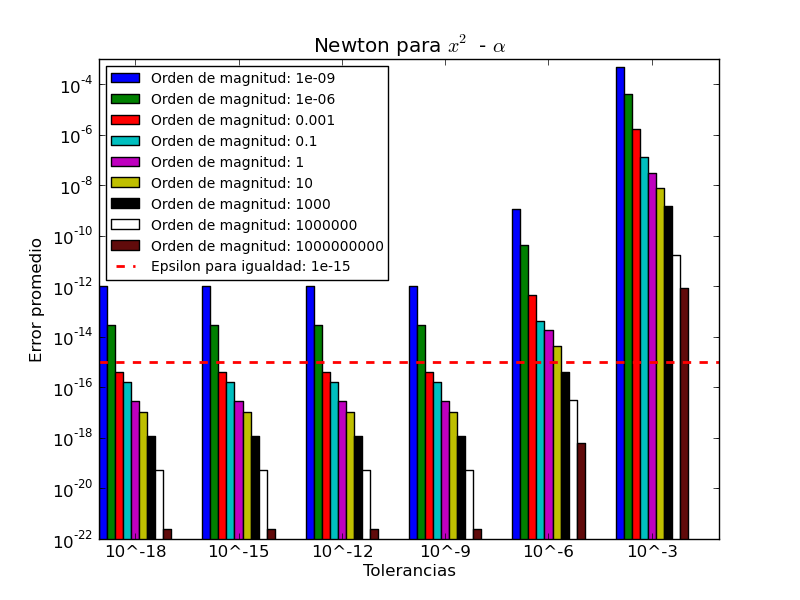
\includegraphics[width=0.9\textwidth]{../data/NewtonF.png}
    \caption{Error relativo final para distintos valores de tolerancia en el criterio de parada utilizando el cero de $x^2-\alpha$ con el método de Newton para cada orden de magnitud medido.}
    \label{paradaMet0}
\end{figure}

Para el primer método, calculamos $z^{-1}$, siendo $z$ un cero de $f(x) = x^2-\alpha$ que obtuvimos mediante el método de Newton. En la figura \ref{paradaMet0} vemos el error relativo final (luego de calculado el cociente) según las distintas tolerancias. Observamos, por un lado, que todos los errores decrecen (no estrictamente) a medida que decrece la tolerancia, lo cual es esperable. Por otro lado, observamos un estancamiento del error para $\tau < 10^{-9}$, con lo cual éste será el valor elegido para este método. Si bien es llamativo que el error no se reduzca para tolerancias menores, sabiendo que el método converge cuadráticamente podemos pensar que el error relativo del criterio de parada se reduce, en una iteración de un valor en el orden de $10^-6$ a uno por debajo de $10^-18$, haciendo que el método termine para todas las tolerancias intermedias al mismo tiempo. Pensamos en investigar qué sucedería para tolerancias menores, pero dado que consideramos como iguales valores que difieran en menos de $10^{-15}$ consideramos que no tenía significación.

Observemos también que el error relativo se hace más significativo cuanto menor es el orden de magnitud, lo que indicaría que el error absoluto no necesariamente acompaña la magnitud de $\alpha$. Atribuimos esto a errores numéricos, que se introducen siempre independientemente del valor representado.


\begin{figure}[H]
  \centering
    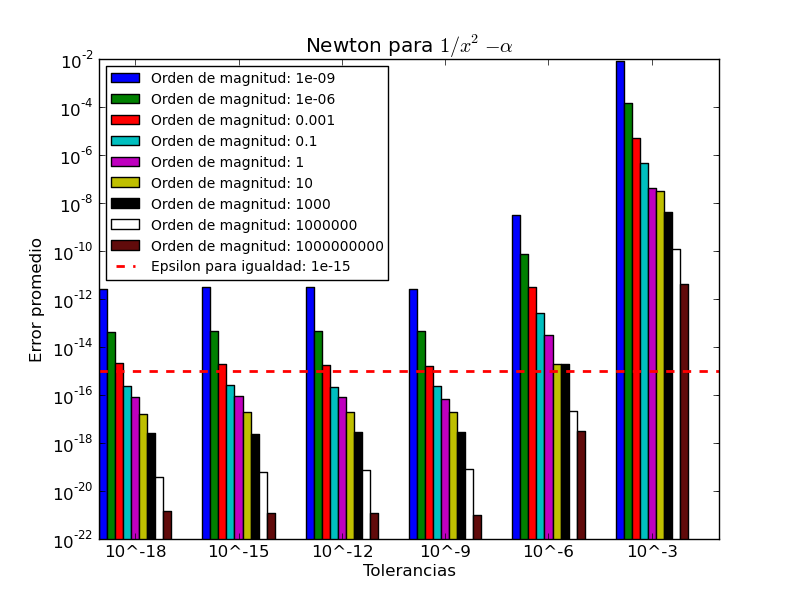
\includegraphics[width=0.9\textwidth]{../data/NewtonE.png}
    \caption{Error relativo final para distintos valores de tolerancia en el criterio de parada para el cero de $\frac{1}{x^2} - \alpha$ con el método de Newton para cada orden de magnitud medido.}
    \label{paradaMet1}
\end{figure}

Observemos que el gráfico es muy similar al de la figura \ref{paradaMet1}, con lo cual, al tratarse del mismo método, caben argumentos similares: el decrecimiento y estancamiento lo atribuimos a la rapidez con la que converge el método y podemos utilizar $10^{-9}$ para el criterio de parada.

\begin{figure}[H]
  \centering
    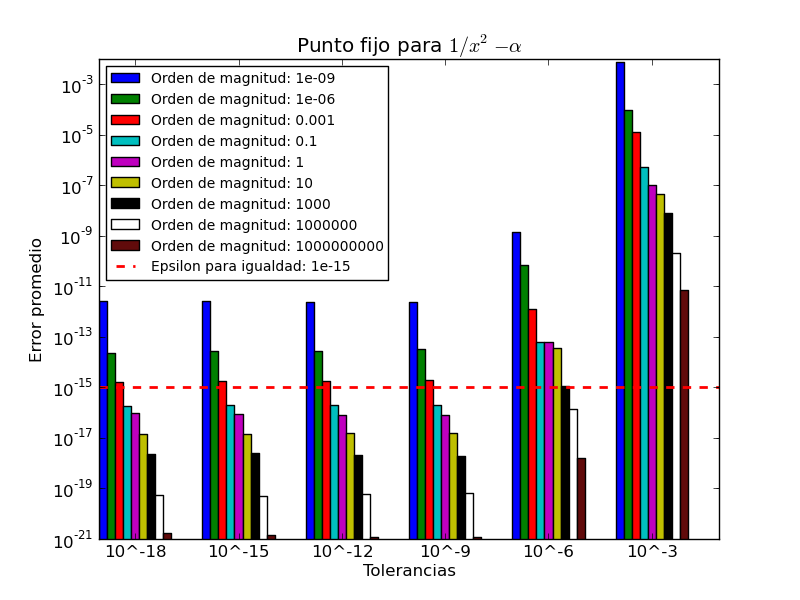
\includegraphics[width=0.9\textwidth]{../data/NewtonPuntoFijo.png}
    \caption{Error relativo final para distintos valores de tolerancia en el criterio de parada para el cero de $\frac{1}{x^2} - \alpha$ con el método de punto fijo para $\frac{1}{\alpha x} + \frac{x - \alpha x^3}{2}$, para cada orden de magnitud medido.}
    \label{paradaMet2}
\end{figure}

Al igual que en el caso anterior, la figura \ref{paradaMet2}, al tratarse de un método cuadrático, admite un análisis análogo a los casos anteriores. En este caso también elegiremos $10^{-9}$.

\begin{figure}[H]
  \centering
    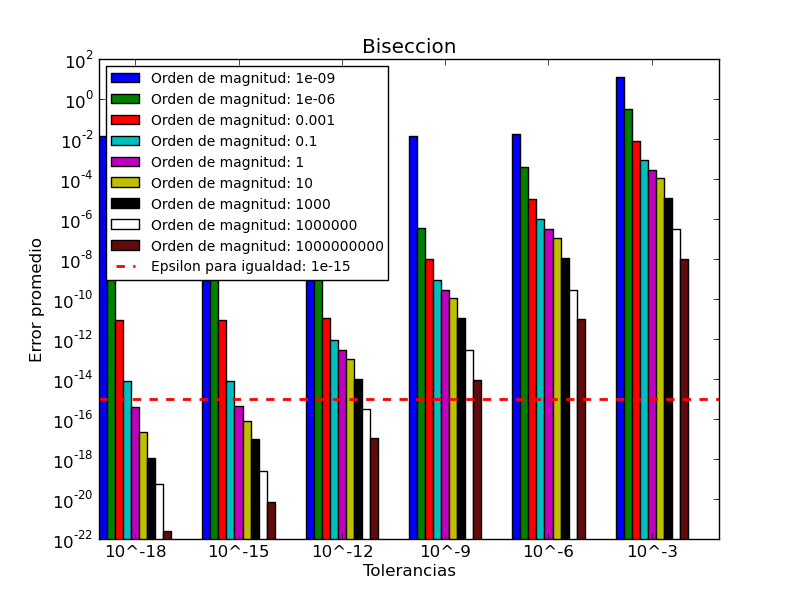
\includegraphics[width=0.9\textwidth]{../data/BiseccionF.png}
    \caption{Error relativo final para distintos valores de tolerancia en el criterio de parada obteniendo el cero de $x^2 - \alpha$ mediante bisección, para cada orden de magnitud medido.}
    \label{paradaMet3}
\end{figure}

Como dijimos, no esperábamos grandes resultados para este método. Elegiremos para seguir $10^{-15}$, que es donde se detiene la reducción del error (nuevamente, relacionado con el criterio de igualdad establecido). Vemos que para los órdenes más pequeños el error relativo es significativo, aún para las tolerancias menores, lo que indica que el error absoluto sigue siendo importante. Sabemos que para $\sqrt{\alpha}$ éste está acotado por la mitad de la longitud del intervalo en el último paso de bisección, que al calcularle el recíproco, tratándose de valores pequeños, éste crece considerablemente.

\subsection{Tiempo de Ejecución}

Para medir tiempo de ejecución, en principio, tomamos los métodos mixtos, sin restricciones sobre la cantidad de bisecciones. En general observamos que los tiempos crecen a medida que el orden de magnitud crece en módulo. Esto está relacionado con los intervalos inciales que elige cada método, que en general están en función de $\alpha$ o $\frac{1}{\alpha}$, según si se trata de valores mayores o menores a uno.
 
\begin{figure}[H]
  \centering
    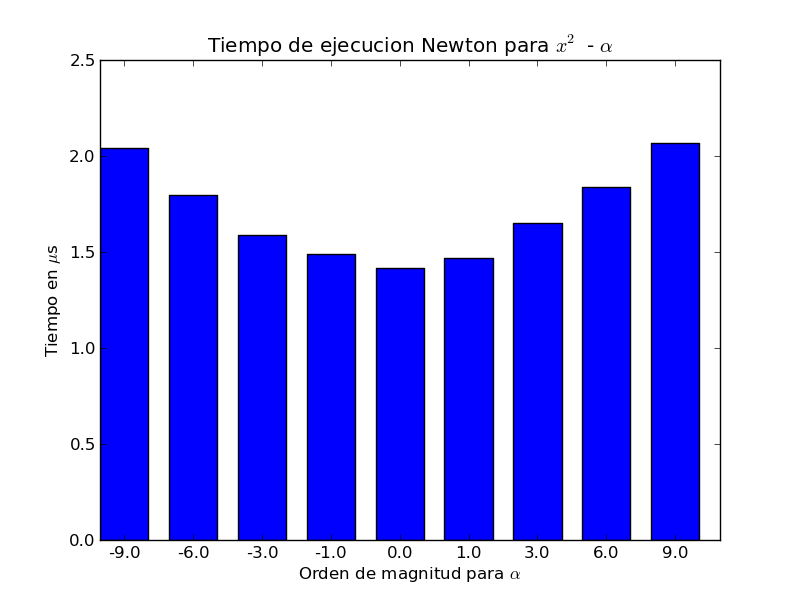
\includegraphics[width=0.9\textwidth]{../data/Tiempometodo0.png}
    \caption{Tiempo de ejecución para el recíproco del cero de $x^2 - \alpha$ con el método de Newton para cada orden de magnitud medido.}
    \label{tiempoMet0}
\end{figure}

Como dijimos, el tiempo de ejecución depende del orden de magnitud. Excepto en los casos extremos, la variación entre el mejor y el peor caso es perfectamente tolerable.

\begin{figure}[H]
  \centering
    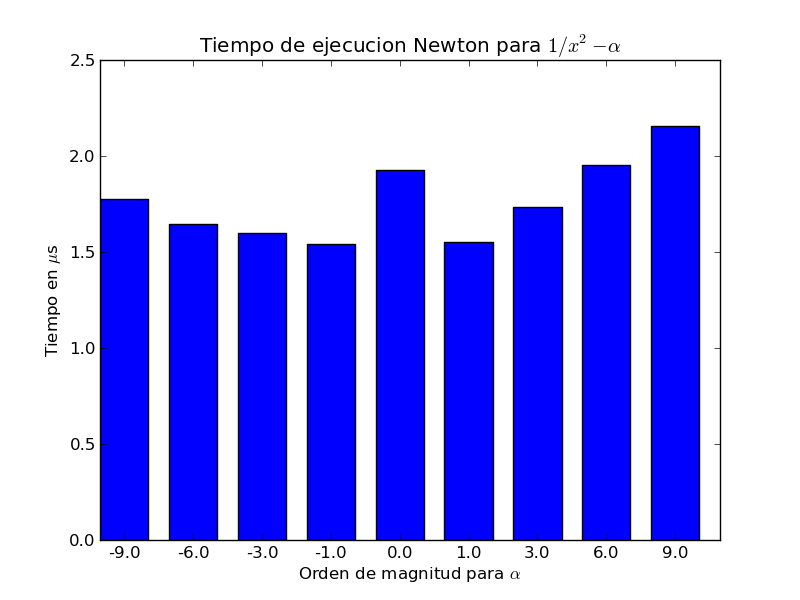
\includegraphics[width=0.9\textwidth]{../data/Tiempometodo1.png}
    \caption{Tiempo de ejecución para el cero de $\frac{1}{x^2} - \alpha$ con el método de Newton para cada orden de magnitud medido.}
    \label{tiempoMet1}
\end{figure}

\begin{figure}[H]
  \centering
    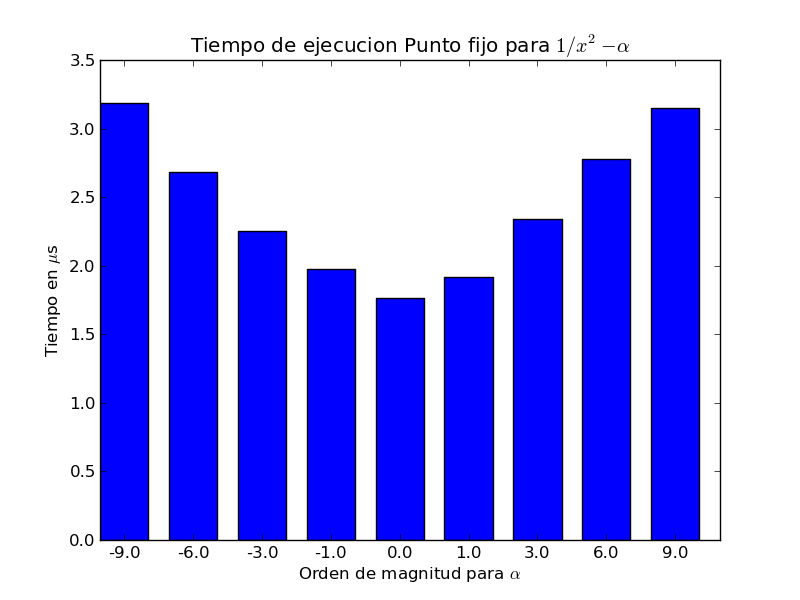
\includegraphics[width=0.9\textwidth]{../data/Tiempometodo2.png}
    \caption{Tiempo de ejecución para el cero de $\frac{1}{x^2} - \alpha$ con el método de punto fijo para cada orden de magnitud medido.}
    \label{tiempoMet2}
\end{figure}

Nuevamente, el tiempo depende del orden de magnitud en el que estamos calculando. Observamos una situación similar a la de la figura \ref{tiempoMet0}, aunque éste método parece más costoso. Esto es esperable si tenemos en cuenta que la función de punto fijo que utiliza contiene más operaciones que la que utilizamos para  el caso anterior.

\begin{figure}[H]
  \centering
    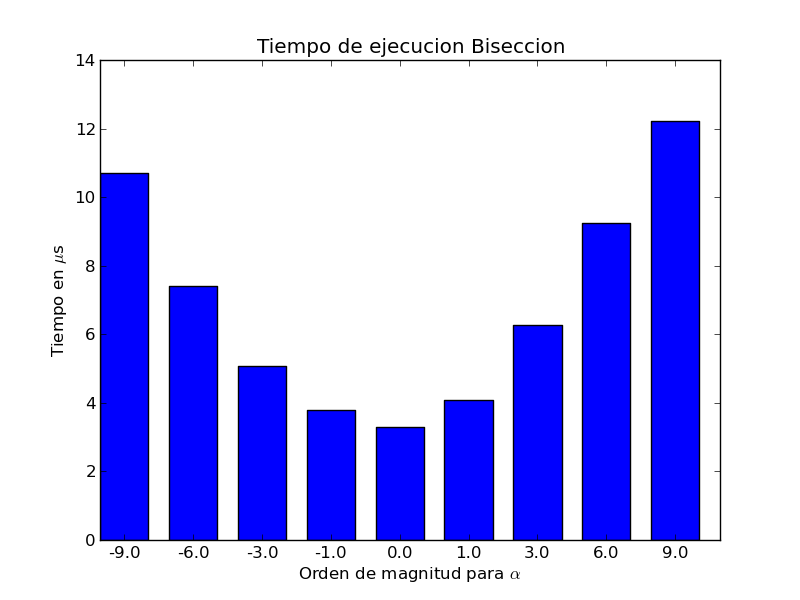
\includegraphics[width=0.9\textwidth]{../data/Tiempometodo3.png}
    \caption{Tiempo de ejecución para el recíproco del cero de ${x^2} - \alpha$ con bisección para cada orden de magnitud medido.}
    \label{tiempoMet3}
\end{figure}

Si bien observamos que la forma general del gráfico es similar a los casos anteriores, si miramos la escala vemos que se trata de un método mucho más lento. Esto es lo que esperábamos, ya que sabemos que converge linealmente, mientras que los otros métodos propuestos los elegimos por tener convergencia cuadrática.

\subsection{Cantidad de iteraciones}
Los siguientes gráficos muestran la cantidad de iteraciones que emplean los distintos métodos para calcular la aproximación a $\frac{1}{\sqrt{\alpha}}$. Dado que cada método realiza una bisección al principio del mismo para reducir el intervalo inicial para garantizar la convergencia, experimentamos restringiendo la cantidad de iteraciones de bisección permitidas para \textquotedblleft relajar\textquotedblright las restricciones que le imponemos al método. Dicho esto, planteamos 3 topes para la cantidad de iteraciones de bisección. Veremos que al no garantizar un intervalo que converja mediante la biseccion, tendremos que dependiendo del tope con el que estemos evaluando, newton convergerá o no. Los topes propuestos son 10, 15 y 20.

\begin{figure}[H]
  \centering
    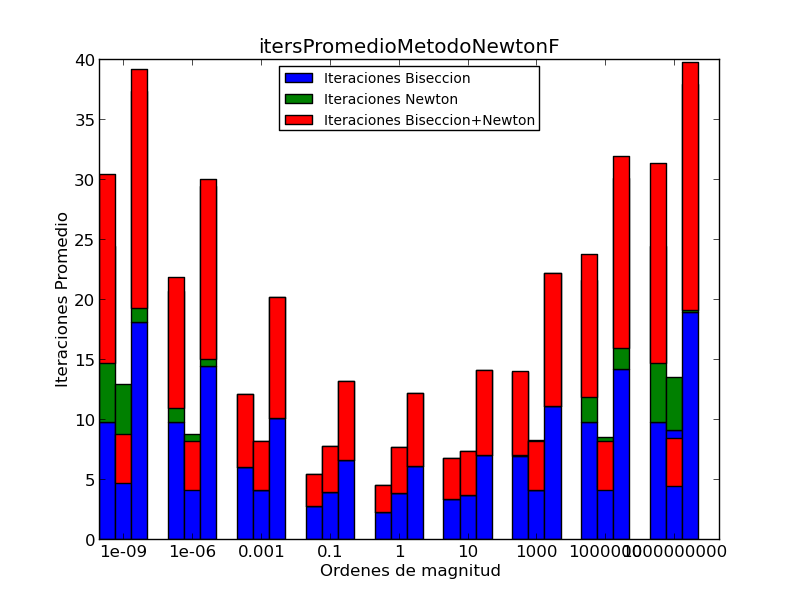
\includegraphics[width=0.9\textwidth]{../data/itersPromedioMetodoNewtonF.png}
    \caption{Iteraciones promedio para el recíproco del cero de ${x^2} - \alpha$ con el método de Newton para cada orden de magnitud medido.}
    \label{iters0}
\end{figure}

Vemos que para cualquier tope de iteraciones de bisección que elijamos, en la figura \ref{iters0} apreciamos que no se superan las 100 iteraciones de Newton, uno de los criterios de parada que propusimos para asegurarnos que los métodos terminan, con lo cual podemos estar seguros que siempre se cumple con la tolerancia propuesta en el criterio de parada.
 Además, vemos que la forma en que varían la cantidad de iteraciones en función es similar a la forma en que lo hace el tiempo de ejecución en la figura \ref{tiempoMet0} como esperábamos.


\begin{figure}[H]
  \centering
    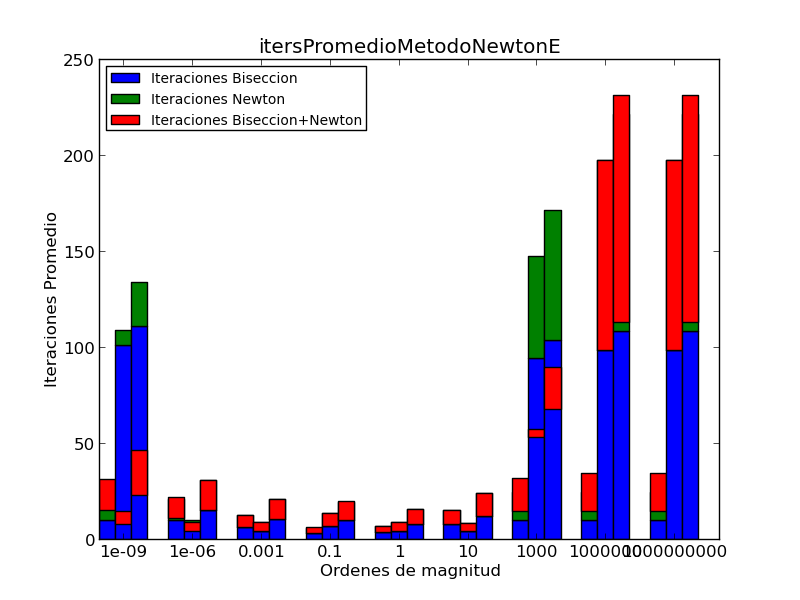
\includegraphics[width=0.9\textwidth]{../data/itersPromedioMetodoNewtonE.png}
    \caption{Iteraciones para el cero de $\frac{1}{x^2} - \alpha$ con el método de Newton para cada orden de magnitud medido.}
    \label{iters1}
\end{figure}

En esta figura empezamos a observar las consecuencias de restringir la cantidad de iteraciones para la bisección inicial. Vemos que para algunos órdenes de magnitud se llega al tope de iteraciones que fijamos para el criterio de parada de Newton y por ende es acertado afirmar que el método no converge. Sin embargo, podemos ver que con 20 iteraciones de bisección Newton converge, el problema sucede con cantidades menores a ésta.

\begin{figure}[H]
  \centering
    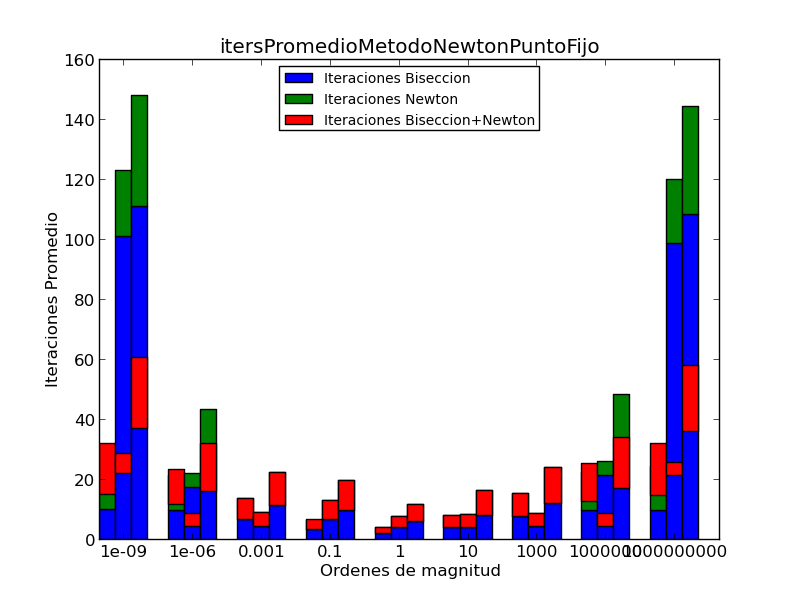
\includegraphics[width=0.9\textwidth]{../data/itersPromedioMetodoNewtonPuntoFijo.png}
    \caption{Tiempo de ejecución para el cero de $\frac{1}{x^2} - \alpha$ con el método de punto fijo para cada orden de magnitud medido.}
    \label{iters2}
\end{figure}

A diferencia de la figura \ref{iters1}, apreciamos que la iteración de punto fijo propuesta para encontrar el cero $\frac{1}{x^2} - \alpha$ tiene más tolerancia a la restricción que se le impone a la cantidad de iteraciones que realiza la bisección al principio del método. Sumado a esto, tomando un tope para el cual el método converge, se realizan menos iteraciones que las que realiza el método de la figura \ref{iters1} con un tope adecuado.


\begin{figure}[H]
  \centering
    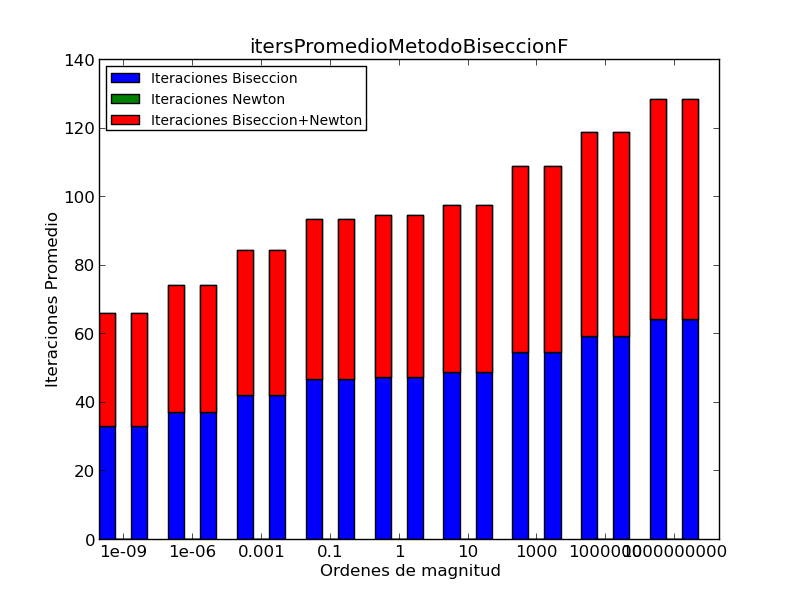
\includegraphics[width=0.9\textwidth]{../data/itersPromedioMetodoBiseccionF.png}
    \caption{Tiempo de ejecución para el recíproco del cero de ${x^2} - \alpha$ con bisección para cada orden de magnitud medido.}
    \label{iters3}
\end{figure}

Cabe destacar que para el método de la bisección no se realizan iteraciones de Newton, por lo que en la figura \ref{iters3} la cantidad de iteraciones para Newton no se ve representada. Como era de esperarse, podemos observar como la cantidad de iteraciones crece linealmente en función del valor de $\alpha$, ya que para todos los $\alpha$ mayores a 1 el intervalo inicial que tomamos para el método de la bisección es igual a $[0,\alpha]$, y este método converge linealmente en función del tamaño del intervalo inicial.





